\section{Оценка сходимости метода сопряженных градиентов для линейной системы с произвольной симметричной положительно определенной матрицей. Случай $\lambda_1 >> \lambda_2$.}

\begin{proposal}
	Для $A = A^\top > 0$ и любого многочлена $h(\lambda): h(0) = 1$ степени $k$ верно:
	$$\|e_k\|_A \le \max_i |h(\lambda_i)|\|e_0\|_A$$
\end{proposal}

В общем случае мы использовали многочлен вида:
$$t_k(\lambda) = \frac{T_k\left(\frac{\lambda_1 + \lambda_n - 2 \lambda}{\lambda_1-\lambda_n}\right)}{T_k\left(\frac{\lambda_1 + \lambda_n}{\lambda_1-\lambda_n}\right)}$$

Где $T_k$ - многочлен Чебышева. Такой $t_k$ меньше всего отклоняется от 0 на отрезке $[\lambda_n, \lambda_1]$, однако чем больше отрезок тем больше мы отклоняемся. Вообще говоря нас интересует отклонение только в точках $\lambda \in \{\lambda_1, \lambda_2, \dots, \lambda_n\}$. Давайте рассмотрим другой многочлен:
$$p_k(\lambda) = \frac{T_{k-1}\left(\frac{\lambda_2 + \lambda_n - 2 \lambda}{\lambda_2-\lambda_n}\right)}{T_{k-1}\left(\frac{\lambda_2 + \lambda_n}{\lambda_2-\lambda_n}\right)}\left(1-\frac{\lambda}{\lambda_1}\right)$$


\begin{center}
	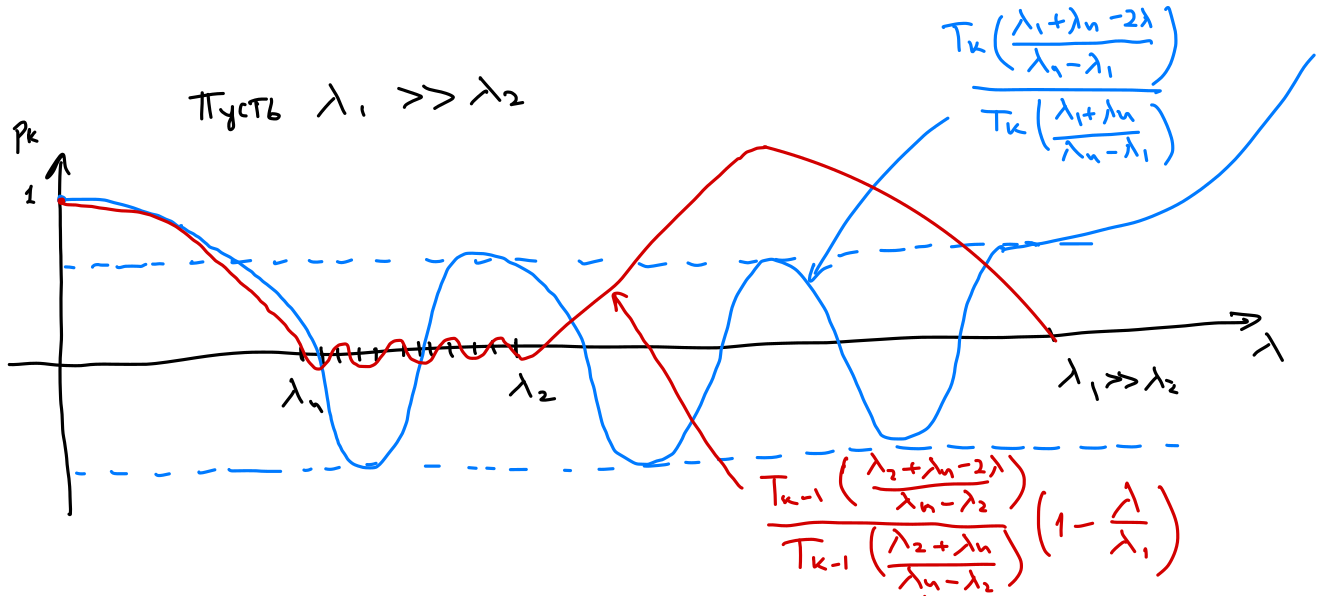
\includegraphics[scale=0.3]{img/q5_1} \\
	(Заметка: на лекции путаница с знаком знаменателя аргумента $T_{i}$)
\end{center}

Тоесть мы уменьшили отрезок, а также пожертвовав степенью многочлена Чебышева, мы добавили множитель который обращается в 0 при $\lambda = \lambda_1$

Нам нужно оценить $\max_i |p_k(\lambda_i)|$, заметим, что:
$$\max_i |p_k(\lambda_i)| \le \max_{\lambda \in [\lambda_{n}, \lambda_2]\cup \{\lambda_1\}}|p_k(\lambda)| = \max_{\lambda \in [\lambda_{n}, \lambda_2]}|p_k(\lambda)|$$

\begin{proposal}
С лекции 14 нам известно:
$$\frac{T_k\left(\frac{a + b - 2 \lambda}{a-b}\right)}{T_k\left(\frac{a + b}{a-b}\right)} \le 2\left(\frac{\sqrt\frac{a}{b} - 1}{\sqrt\frac{a}{b} + 1}\right)^k$$
\end{proposal}

Теперь оценим $p_k$ на множестве $[\lambda_{n}, \lambda_2]$:

\begin{flalign}
	p_k(\lambda) = \frac{T_{k-1}\left(\frac{\lambda_2 + \lambda_n - 2 \lambda}{\lambda_2-\lambda_n}\right)}{T_{k-1}\left(\frac{\lambda_2 + \lambda_n}{\lambda_2-\lambda_n}\right)}\left(1-\frac{\lambda}{\lambda_1}\right) \le 2\left(1-\frac{\lambda}{\lambda_1}\right)\left(\frac{\sqrt\frac{\lambda_2}{\lambda_n} - 1}{\sqrt\frac{\lambda_2}{\lambda_n} + 1}\right)^{k-1} \le 2\left(1-\frac{\lambda_n}{\lambda_1}\right)\left(\frac{\sqrt\frac{\lambda_2}{\lambda_n} - 1}{\sqrt\frac{\lambda_2}{\lambda_n} + 1}\right)^{k-1}
\end{flalign}

Осталось заметить, что $1-\frac{\lambda_n}{\lambda_1} \le 1$, тогда:
$$p_k(\lambda) \le 2\left(1-\frac{\lambda_n}{\lambda_1}\right)\left(\frac{\sqrt\frac{\lambda_2}{\lambda_n} - 1}{\sqrt\frac{\lambda_2}{\lambda_n} + 1}\right)^{k-1} \le 2\left(\frac{\sqrt\frac{\lambda_2}{\lambda_n} - 1}{\sqrt\frac{\lambda_2}{\lambda_n} + 1}\right)^{k-1}$$

Используя первое предложение можно сделать вывод:
$$\|e_k\|_A \le 2\left(\frac{\sqrt\frac{\lambda_2}{\lambda_n} - 1}{\sqrt\frac{\lambda_2}{\lambda_n} + 1}\right)^{k-1}\|e_0\|_A$$
